
\section*{CHƯƠNG 3. THIẾT KẾ HỆ THỐNG}
\setcounter{section}{3}
\setcounter{subsection}{0} %LƯU Ý MỖI LẦN THÊM CHƯƠNG MỚI CẦN THÊM CÂU NÀY ĐỂ RESET THỨ TỰ CỦA SUBSECTON VỀ 1
\setcounter{table}{0} % LƯU Ý SAU MỖI LẦN GỌI BẢNG HAY HÌNH ẢNH PHẢI THÊM CÂU NÀY ĐỂ RESET THỨ TỰ
\setcounter{figure}{0} %% LƯU Ý SAU MỖI LẦN GỌI BẢNG HAY HÌNH ẢNH PHẢI THÊM CÂU NÀY ĐỂ RESET THỨ TỰ
\addcontentsline{toc}{section}{\numberline{}CHƯƠNG 3. THIẾT KẾ HỆ THỐNG}

Trong chương này, chúng em sẽ trình bày về thiết kế hệ thống từ tổng quan đến chi tiết dựa trên phân tích từ Chương 2. Bắt đầu với việc xây dựng sơ đồ kiến trúc hệ thống,
sau đó là thiết kế giao diện, chức năng cho website và server. Nội dung chính của chương sẽ tập trung vào các hình
ảnh và sơ đồ mô tả chi tiết từng luồng hoạt động của hệ thống và đồng thời minh họa cách các phần trong hệ thống tương tác với nhau.

\subsection{Sơ đồ kiến trúc tổng quan của hệ thống}
Hệ thống được chia làm ba phần chính bao gồm Device (Thiết bị), Server (Máy chủ) và Application (Ứng dụng bao gồm: web và app). Mỗi thành phần đóng vai trò quan trọng trong việc vận hành tổng thể hệ thống trong hình vẽ:

% \begin{figure}[H]
%   \centering
%   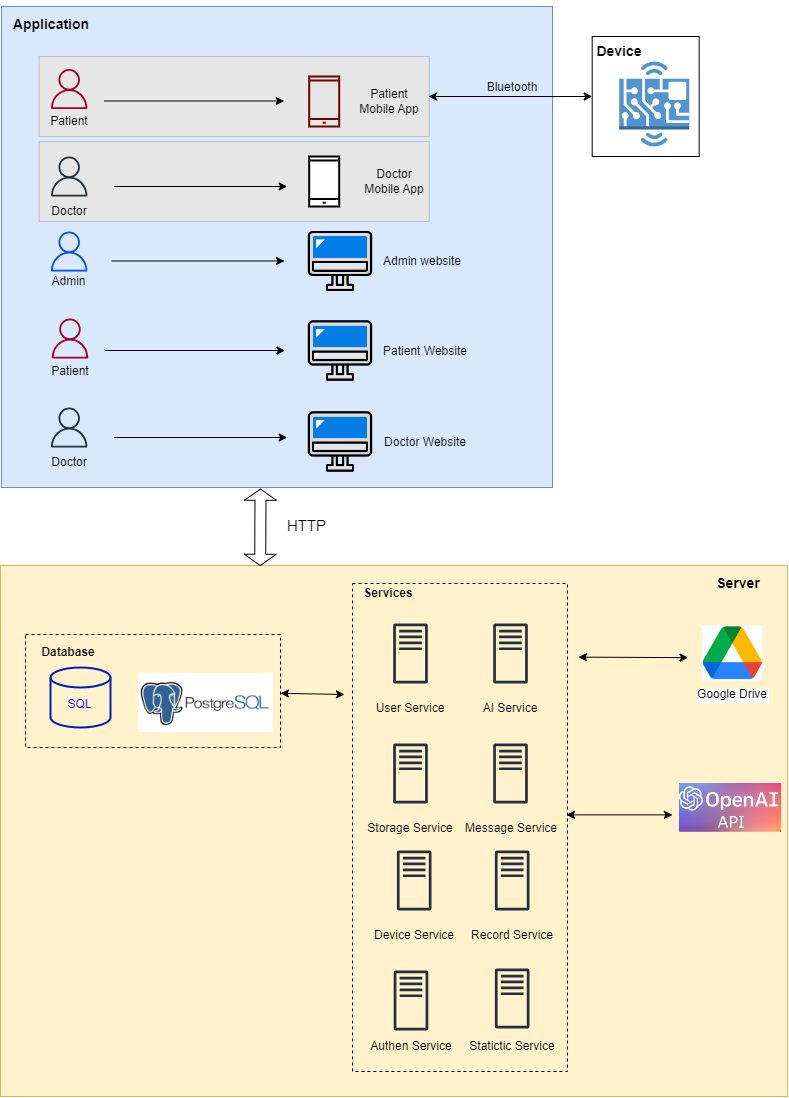
\includegraphics[width=12cm,height=14cm]{Images/system/fmECG_architecture-System_Architecture.png}
%   \caption[Kiến trúc tổng quan hệ thống]{\bfseries \fontsize{12pt}{0pt}\selectfont Kiến trúc tổng quan hệ thống}
%   \label{fmECG_architecture-System} %đặt tên cho ảnh
% \end{figure}

Hình  thể hiện ba phần: 

\begin{adjustwidth}{1.5em}{}
\begin{itemize}
  \item Device (Thiết bị): Bao gồm thiết bị phần cứng đo điện tim, có thể kết nối với ứng dụng di động của bệnh nhân thông qua Bluetooth 
  \item Application (Ứng dụng): Bao gồm ứng dụng di động cho bệnh nhân, bác sĩ; website của quản trị viên, website của bác sĩ, website của bệnh nhân
  \item Server (Máy chủ): Bao gồm các Services để xử lý các yêu cầu gửi từ Application, cơ sở dữ liệu, Cloud lưu trữ, kết nối với model GPT-4 trên OpenAI thông qua API
\end{itemize}
\end{adjustwidth}

Trong sơ đồ kiến trúc hệ thống, bệnh nhân tương tác trực tiếp với Thiết bị (Device) thông qua ứng dụng di động (Mobile App). Khối Ứng dụng (Application) giao tiếp với Khối Máy chủ (Server) thông qua API với giao thức HTTP. 
Khi nhận được yêu cầu từ Application, Server sẽ xử lý dữ liệu. Mọi yêu cầu đều được xử lý bởi các Services chuyên biệt. Dựa vào loại yêu cầu, Service tương ứng sẽ lấy hoặc lưu dữ liệu trong cơ sở dữ liệu và trả về kết quả cho người dùng.\begin{adjustwidth}{1.5em}{}
\begin{itemize}
  \item User Service: Xử lý các yêu cầu liên quan đến người dùng như đăng ký, đăng nhập, lấy thông tin cá nhân
  \item Storage Service: Xử lý các tác vụ liên quan tới lưu trữ dữ liệu của hệ thống
  \item AI Service: Xử lý các tác vụ liên quan tới trợ lý ảo, bao gồm: huấn luyện, kết nối với model GPT-4 thông qua api và xử lý kết quả 
  và trả về tin nhắn và các hành động của ai can thiệp trực tiếp vào hệ thống 
  \item Message Service: Xử lý các yêu cầu liên quan tới hội thoại, tin nhắn.
  \item Device Service: Xử lý các tác vụ liên quan tới thiết bị như thêm, sửa, xoá thiết bị, cập nhật thông tin.
  \item Record Service: Xử lý các tác vụ liên quan tới bản ghi như là thêm sửa xoá, xử lý dữ liệu file đo, vẽ đồ thị
  \item Authen Service: Xử lý các tác vụ liên quan tới bảo mật như: mã hoá và cung cấp token, kiểm tra token, phân quyền truy cập api, mã hoá các dữ liệu nhạy cảm trước khi lưu trữ.
  \item Statictic Service: Xử lý các tác vụ liên quan tới thống kê như: thống kê người dùng, thiết bị, bản ghi, tin nhắn theo tuần theo tháng.
\end{itemize}
\end{adjustwidth}

Ngoài ra hệ thống sẽ có thêm chức năng tự động triển khai trên môi trường internet để việc phát triển và kiểm thử dễ dàng 
làm tăng chất lượng và độ hoàn thiện của hệ thống.

Sau đây là mô tả chi tiết về từng khối nhỏ hơn trong kiến trúc hệ thống, dựa trên các đối tượng đã được xác định trong hệ thống.
\newpage
\subsection{Sơ đồ khối phần mềm}

\subsubsection{Website dành cho bệnh nhân}



\subsubsection{Website dành cho bác sĩ}


\subsubsection{Website cho quản trị viên}


\subsection{Thiết kế cơ sở dữ liệu}

\subsubsection{Chuẩn hoá 3NF}
Các bảng đã được thiết kế theo nguyên tắc chuẩn hoá 3NF, vì không có thuộc tính lặp lại và các thuộc tính không phụ thuộc vào một tập hợp con của khóa chính.

\paragraph{Chuẩn hoá bảng Người dùng}
\mbox{}
\begin{table}[H]
  \caption{\bfseries \fontsize{12pt}{0pt}\selectfont Bảng chuẩn hoá bảng Người dùng}
  \centering
  \begin{tabularx}{0.9\textwidth}{|X|X|}
    \hline
    \textbf{Danh sách thuộc tính} & ID người dùng, ID tài khoản, Tên người dùng, Ngày sinh, Giới tính, Số điện thoại, Quyền, Trạng thái, Đường dẫn lưu trữ ảnh, Thông tin người dùng \\
    \hline
    \textbf{Quy tắc nghiệp vụ} & \textbf{Phụ thuộc hàm} \\
    \hline
    Mỗi người dùng có một ID riêng, có duy nhất ID tài khoản, tên, ngày sinh, giới tính, số điện thoại, quyền,
    trạng thái, đường dẫn lưu trữ ảnh, thông tin & \parbox[t]{\linewidth}{$\text{ID người dùng} \rightarrow$ ID tài khoản, Tên người dùng, Ngày sinh, Giới Tính, Số điện thoại, Quyền, Trạng thái, Đường dẫn lưu trữ ảnh, Thông tin} \\
    \hline
    \multicolumn{2}{|X|}{$\Rightarrow \text{Khoá chính của bảng: ID người dùng}$} \\
    \multicolumn{2}{|X|}{$\Rightarrow \text{Bảng Người dùng đã ở 3NF}$} \\
    \hline
  \end{tabularx}
\end{table}

\paragraph{Chuẩn hoá bảng Tài khoản}
\mbox{}
\begin{table}[H]
  \caption{\bfseries \fontsize{12pt}{0pt}\selectfont Bảng chuẩn hoá bảng Tài khoản}
  \centering
  \begin{tabularx}{0.9\textwidth}{|X|X|}
    \hline
    \textbf{Danh sách thuộc tính} & ID tài khoản, Email, Mật khẩu \\
    \hline
    \textbf{Quy tắc nghiệp vụ} & \textbf{Phụ thuộc hàm} \\
    \hline
    Mỗi tài khoản có một ID riêng, có duy nhất email, mật khẩu 
    & \parbox[t]{\linewidth}{$\text{ID tài khoản} \rightarrow$ Email, mật khẩu} \\
    \hline
    \multicolumn{2}{|X|}{$\Rightarrow \text{Khoá chính của bảng: ID tài khoản}$} \\
    \multicolumn{2}{|X|}{$\Rightarrow \text{Bảng Tài khoản đã ở 3NF}$} \\
    \hline
  \end{tabularx}
\end{table}

\paragraph{Chuẩn hoá bảng Token đăng nhập}
\mbox{}
\begin{table}[H]
  \caption{\bfseries \fontsize{12pt}{0pt}\selectfont Bảng chuẩn hoá bảng Token đăng nhập}
  \centering
  \begin{tabularx}{0.9\textwidth}{|X|X|}
    \hline
    \textbf{Danh sách thuộc tính} & ID token, ID tài khoản, Token truy cập, Token làm mới \\
    \hline
    \textbf{Quy tắc nghiệp vụ} & \textbf{Phụ thuộc hàm} \\
    \hline
    Mỗi người dùng có một ID token riêng, có duy nhất ID tài khoản, token truy cập và token làm mới 
    & \parbox[t]{\linewidth}{$\text{ID token} \rightarrow$ ID tài khoản, Token truy cập, Token làm mới} \\
    \hline
    \multicolumn{2}{|X|}{$\Rightarrow \text{Khoá chính của bảng: ID token đăng nhập}$} \\
    \multicolumn{2}{|X|}{$\Rightarrow \text{Bảng Token  đã ở 3NF}$} \\
    \hline
  \end{tabularx}
\end{table}

\paragraph{Chuẩn hoá bảng Thiết bị}
\mbox{}
\begin{table}[H]
  \caption{\bfseries \fontsize{12pt}{0pt}\selectfont Bảng chuẩn hoá bảng Thiết bị}
  \centering
  \begin{tabularx}{0.9\textwidth}{|X|X|}
    \hline
    \textbf{Danh sách thuộc tính} & ID thiết bị, ID người dùng thiết bị, ID bác sĩ theo dõi, Tên thiết bị, 
    Loại thiết bị, Thông tin thiết bị, Trạng thái thiết bị, Ngày bắt đầu sử dụng \\
    \hline
    \textbf{Quy tắc nghiệp vụ} & \textbf{Phụ thuộc hàm} \\
    \hline
    Mỗi thiết bị khi được sử dụng sẽ có một ID thiết bị riêng, có duy nhất tên thiết bị, loại thiết bị, thông tin thiết bị.
    ID người dùng thiết bị, ID bác sĩ theo dõi, trạng thái thiết bị, ngày bắt đầu sử dụng
    & \parbox[t]{\linewidth}{$\text{ID thiết bị} \rightarrow$ ID người dùng thiết bị, ID bác sĩ theo dõi, Tên thiết bị, 
    Loại thiết bị, Thông tin thiết bị, Trạng thái thiết bị, Ngày bắt đầu sử dụng} \\
    \hline
    \multicolumn{2}{|X|}{$\Rightarrow \text{Khoá chính của bảng: ID thiết bị}$} \\
    \multicolumn{2}{|X|}{$\Rightarrow \text{Bảng Thiết bị đã ở 3NF}$} \\
    \hline
  \end{tabularx}
\end{table}

\paragraph{Chuẩn hoá bảng Thông số thiết bị}
\mbox{}
\begin{table}[H]
  \caption{\bfseries \fontsize{12pt}{0pt}\selectfont Bảng chuẩn hoá bảng Thông số thiết bị}
  \centering
  \begin{tabularx}{0.9\textwidth}{|X|X|}
    \hline
    \textbf{Danh sách thuộc tính} & ID thông số, ID thiết bị, Tên thông số, Giá trị, 
    Thông tin thông số, Loại thông số \\
    \hline
    \textbf{Quy tắc nghiệp vụ} & \textbf{Phụ thuộc hàm} \\
    \hline
    Mỗi thông số thiết bị sẽ có một ID thông số riêng, có duy nhất Tên thông số, ID thiết bị, Giá trị,
    Thông tin thông số, Loại thông số
    & \parbox[t]{\linewidth}{$\text{ID thông số} \rightarrow$ Tên thông số, ID thiết bị, Giá trị,
    Thông tin thông số, Loại thông số} \\
    \hline
    \multicolumn{2}{|X|}{$\Rightarrow \text{Khoá chính của bảng: ID thông số thiết bị}$} \\
    \multicolumn{2}{|X|}{$\Rightarrow \text{Bảng Thiết bị đã ở 3NF}$} \\
    \hline
  \end{tabularx}
\end{table}

\paragraph{Chuẩn hoá bảng Bản ghi dữ liệu}
\mbox{}
\begin{table}[H]
  \caption{\bfseries \fontsize{12pt}{0pt}\selectfont Bảng chuẩn hoá bảng Bản ghi dữ liệu}
  \centering
  \begin{tabularx}{0.9\textwidth}{|X|X|}
    \hline
    \textbf{Danh sách thuộc tính} & ID bản ghi dữ liệu, ID người dùng, ID thiết bị, Loại bản ghi, 
    Đường dẫn lưu trữ dữ liệu, Thời gian bắt đầu đo, Thời gian kết thúc đo \\
    \hline
    \textbf{Quy tắc nghiệp vụ} & \textbf{Phụ thuộc hàm} \\
    \hline
    Mỗi bản ghi có một ID bản ghi dữ liệu riêng, có duy nhất ID người dùng, ID thiết bị, Loại bản ghi, 
    Đường dẫn lưu trữ dữ liệu, Thời gian bắt đầu đo, Thời gian kết thúc đo
    & \parbox[t]{\linewidth}{$\text{ID bản ghi dữ liệu} \rightarrow$ ID người dùng, ID thiết bị, Loại bản ghi, 
    Đường dẫn lưu trữ dữ liệu, Thời gian bắt đầu đo, Thời gian kết thúc đo} \\
    \hline
    \multicolumn{2}{|X|}{$\Rightarrow \text{Khoá chính của bảng: ID bản ghi dữ liệu}$} \\
    \multicolumn{2}{|X|}{$\Rightarrow \text{Bảng Bản ghi dữ liệu đã ở 3NF}$} \\
    \hline
  \end{tabularx}
\end{table}

\paragraph{Chuẩn hoá bảng Thông tin hội thoại}
\mbox{}
\begin{table}[H]
  \caption{\bfseries \fontsize{12pt}{0pt}\selectfont Bảng chuẩn hoá bảng Thông tin hội thoại}
  \centering
  \begin{tabularx}{0.9\textwidth}{|X|X|}
    \hline
    \textbf{Danh sách thuộc tính} & ID hội thoại, Tên hội thoại, 
    Loại hội thoại, Đường dẫn avatar hội thoại \\
    \hline
    \textbf{Quy tắc nghiệp vụ} & \textbf{Phụ thuộc hàm} \\
    \hline
    Mỗi hội thoại có một ID hội thoại riêng, có duy nhất tên hội thoại, 
    loại hội thoại, đường dẫn avatar hội thoại
    & \parbox[t]{\linewidth}{$\text{ID hội thoại} \rightarrow$ Tên hội thoại, 
    Loại hội thoại, Đường dẫn avatar hội thoại} \\
    \hline
    \multicolumn{2}{|X|}{$\Rightarrow \text{Khoá chính của bảng: ID hội thoại}$} \\
    \multicolumn{2}{|X|}{$\Rightarrow \text{Bảng Thông tin hội thoại đã ở 3NF}$} \\
    \hline
  \end{tabularx}
\end{table}

\paragraph{Chuẩn hoá bảng Thành viên tham gia hội thoại}
\mbox{}
\begin{table}[H]
  \caption{\bfseries \fontsize{12pt}{0pt}\selectfont Bảng chuẩn hoá bảng Thành viên tham gia hội thoại}
  \centering
  \begin{tabularx}{0.9\textwidth}{|X|X|}
    \hline
    \textbf{Danh sách thuộc tính} & ID, ID hội thoại, ID người dùng tham gia,
    Trạng thái thông báo, Tác vụ, Trạng thái đã xem \\
    \hline
    \textbf{Quy tắc nghiệp vụ} & \textbf{Phụ thuộc hàm} \\
    \hline
    Mỗi hội thoại có nhiều ID người dùng tham gia, mỗi người dùng có duy nhất trạng thái thông báo,
    tác vụ, trạng thái đã xem trong một hội thoại
    & \parbox[t]{\linewidth}{$\text{ID} \rightarrow$ ID hội thoại, ID người dùng tham gia,
    Trạng thái thông báo, Tác vụ, Trạng thái đã xem} \\
    \hline
    \multicolumn{2}{|X|}{$\Rightarrow \text{Khoá chính của bảng: ID}$} \\
    \multicolumn{2}{|X|}{$\Rightarrow \text{Bảng Thành viên tham gia hội thoại đã ở 3NF}$} \\
    \hline
  \end{tabularx}
\end{table}

\paragraph{Chuẩn hoá bảng Tin nhắn}
\mbox{}
\begin{table}[H]
  \caption{\bfseries \fontsize{12pt}{0pt}\selectfont Bảng chuẩn hoá bảng Tin nhắn}
  \centering
  \begin{tabularx}{0.9\textwidth}{|X|X|}
    \hline
    \textbf{Danh sách thuộc tính} & ID tin nhắn, ID hội thoại, ID người gửi, Các tệp đính kèm, 
    Tin nhắn hệ thống, Ghim, Thời gian ghim tin nhắn, Các lượt thả cảm xúc \\
    \hline
    \textbf{Quy tắc nghiệp vụ} & \textbf{Phụ thuộc hàm} \\
    \hline
    Mỗi tin nhắn có một ID tin nhắn riêng, thuộc một hội thoại, có duy nhất ID người gửi, các tệp đính kèm,
    tin nhắn hệ thống, ghim, thời gian ghim tin nhắn, các lượt thả cảm xúc
    & \parbox[t]{\linewidth}{$\text{ID tin nhắn} \rightarrow$ ID hội thoại, ID người gửi, các tệp đính kèm,
    tin nhắn hệ thống, ghim, thời gian ghim tin nhắn, các lượt thả cảm xúc} \\
    \hline
    \multicolumn{2}{|X|}{$\Rightarrow \text{Khoá chính của bảng: ID tin nhắn}$} \\
    \multicolumn{2}{|X|}{$\Rightarrow \text{Bảng Tin nhắn đã ở 3NF}$} \\
    \hline
  \end{tabularx}
\end{table}

\paragraph{Chuẩn hoá bảng Tệp đính kèm}
\mbox{}
\begin{table}[H]
  \caption{\bfseries \fontsize{12pt}{0pt}\selectfont Bảng chuẩn hoá bảng Tệp đính kèm}
  \centering
  \begin{tabularx}{0.9\textwidth}{|X|X|}
    \hline
    \textbf{Danh sách thuộc tính} & ID tệp đính kèm, ID tin nhắn, ID hội thoại, Đường dẫn nội
    dung, Tên tệp, Kích thước tệp, Đường dẫn thumbnail, Loại đính kèm \\
    \hline
    \textbf{Quy tắc nghiệp vụ} & \textbf{Phụ thuộc hàm} \\
    \hline
    Mỗi tệp đính kèm có một ID tệp đính kèm riêng, thuộc một tin nhắn trong một hội thoại, có duy nhất đường dẫn nội
    dung, tên tệp, kích thước tệp, đường dẫn thumbnail, loại đính kèm
    & \parbox[t]{\linewidth}{$\text{ID tệp đính kèm} \rightarrow$ ID tin nhắn, ID hội thoại, Đường dẫn nội
    dung, Tên tệp, Kích thước tệp, Đường dẫn thumbnail, Loại đính kèm} \\
    \hline
    \multicolumn{2}{|X|}{$\Rightarrow \text{Khoá chính của bảng: ID tệp đính kèm}$} \\
    \multicolumn{2}{|X|}{$\Rightarrow \text{Bảng Tệp đính kèm đã ở 3NF}$} \\
    \hline
  \end{tabularx}
\end{table}

\paragraph{Chuẩn hoá bảng Phân công bệnh nhân - bác sĩ}
\mbox{}
\begin{table}[H]
  \caption{\bfseries \fontsize{12pt}{0pt}\selectfont Bảng chuẩn hoá bảng Phân công bệnh nhân - bác sĩ}
  \centering
  \begin{tabularx}{0.9\textwidth}{|X|X|}
    \hline
    \textbf{Danh sách thuộc tính} & ID phân công, ID bệnh nhân, ID bác sĩ, Ngày bắt đầu \\
    \hline
    \textbf{Quy tắc nghiệp vụ} & \textbf{Phụ thuộc hàm} \\
    \hline
    Mỗi phân công bệnh nhân - bác sĩ có một ID phân công riêng, có duy nhất ID bệnh nhân, ID bác sĩ, ngày bắt đầu.
    Mỗi bệnh nhân thuộc một phân công duy nhất, còn mỗi bác sĩ có thể được giao nhiều phân công.
    & \parbox[t]{\linewidth}{$\text{ID phân công} \rightarrow$ ID bệnh nhân, ID bác sĩ, Ngày bắt đầu} \\
    \hline
    \multicolumn{2}{|X|}{$\Rightarrow \text{Khoá chính của bảng: ID phân công}$} \\
    \multicolumn{2}{|X|}{$\Rightarrow \text{Bảng Phân công bệnh nhân - bác sĩ đã ở 3NF}$} \\
    \hline
  \end{tabularx}
\end{table}

\paragraph{Chuẩn hoá bảng Tài khoản phê duyệt}
\mbox{}
\begin{table}[H]
  \caption{\bfseries \fontsize{12pt}{0pt}\selectfont Bảng chuẩn hoá bảng Tài khoản phê duyệt}
  \centering
  \begin{tabularx}{0.9\textwidth}{|X|X|}
    \hline
    \textbf{Danh sách thuộc tính} & ID tài khoản phê duyệt, Email, Mật khẩu, Tên người dùng, Ngày sinh, Giới tính, Số điện thoại, Quyền, Trạng thái, Đường dẫn lưu trữ ảnh, Thông tin người dùng \\
    \hline
    \textbf{Quy tắc nghiệp vụ} & \textbf{Phụ thuộc hàm} \\
    \hline
    Mỗi tài khoản chờ phê duyệt có một ID riêng, có duy nhất Email, Mật khẩu, Tên người dùng, Ngày sinh, Giới tính,
     Số điện thoại, Quyền, Trạng thái, Đường dẫn lưu trữ ảnh, Thông tin người dùng 
    & \parbox[t]{\linewidth}{$\text{ID tài khoản phê duyệt} \rightarrow$ Email, Mật khẩu, Tên người dùng, Ngày sinh, Giới tính,
    Số điện thoại, Quyền, Trạng thái, Đường dẫn lưu trữ ảnh, Thông tin người dùng} \\
    \hline
    \multicolumn{2}{|X|}{$\Rightarrow \text{Khoá chính của bảng: ID tài khoản phê duyệt}$} \\
    \multicolumn{2}{|X|}{$\Rightarrow \text{Bảng Người dùng đã ở 3NF}$} \\
    \hline
  \end{tabularx}
\end{table}

\subsubsection{Từ điển dữ liệu}

\begin{table}[H]
  \caption{\bfseries \fontsize{12pt}{0pt}\selectfont Bảng user}
  \centering
  \begin{tabularx}{\textwidth}{|c|c|X|}
    \hline
    \textbf{Thuộc tính} & \textbf{Kiểu dữ liệu} & \textbf{Mô tả} \\
    \hline
    id & STRING & ID người dùng.  \\
    \hline
    account\_id & STRING & ID tài khoản người dùng. \\
    \hline
    username & STRING & Họ và tên người dùng. \\
    \hline
    gender & INT & Giới tính của người dùng. \\
    \hline
    birth & DATE & Ngày tháng năm sinh của người dùng. \\
    \hline
    phone\_number & STRING & Số điện thoại của người dùng. \\
    \hline
    image & STRING & Ảnh đại diện của người dùng. \\
    \hline
    status & INTEGER & Trạng thái sử dụng của người dùng (0 - còn đang sử dụng, 1 - không còn đang sử dụng). \\
    \hline
    information & STRING & Thông tin thêm về người dùng. \\
    \hline
    role & INTEGER & Chức vụ của người dùng (0 - bệnh nhân, 1 - bác sĩ, 2 - quản trị viên). \\
    \hline
    created\_at & DATE & Thời gian lúc tạo mới dữ liệu trong cơ sở dữ liệu. \\
    \hline
    updated\_at & DATE & Thời gian lúc thay đổi dữ liệu trong cơ sở dữ liệu. \\
    \hline
    
  \end{tabularx}
\end{table}


\begin{table}[H]
  \caption{\bfseries \fontsize{12pt}{0pt}\selectfont Bảng account}
  \centering
  \begin{tabularx}{\textwidth}{|c|c|X|}
    \hline
    \textbf{Thuộc tính} & \textbf{Kiểu dữ liệu} & \textbf{Mô tả} \\
    \hline
    id & STRING & ID tài khoản  \\
    \hline
    email & STRING & Địa chỉ email của tài khoản. \\
    \hline
    password & STRING & Mật khẩu của tài khoản. \\
    \hline
  \end{tabularx}
\end{table}

\begin{table}[H]
  \caption{\bfseries \fontsize{12pt}{0pt}\selectfont Bảng register}
  \centering
  \begin{tabularx}{\textwidth}{|c|c|X|}
    \hline
    \textbf{Thuộc tính} & \textbf{Kiểu dữ liệu} & \textbf{Mô tả} \\
    \hline
    id & STRING & ID tài khoản đăng ký \\
    \hline
    email & STRING & Địa chỉ email của tài khoản đăng ký. \\
    \hline
    password & STRING & Mật khẩu của tài khoản đâng ký. \\
    \hline
    username & STRING & Họ và tên của tài khoản đăng ký. \\
    \hline
    gender & INT & Giới tính của tài khoản đăng ký. \\
    \hline
    birth & DATE & Ngày sinh của tài khoản đăng ký. \\
    \hline
    phone\_number & STRING & Số điện thoại của tài khoản đăng ký. \\
    \hline
    image & STRING & Ảnh đại diện của tài khoản đăng ký. \\
    \hline
    status & INTEGER & Trạng thái của tài khoản đăng ký (0 - đang chờ xử lý, 1 - được admin chấp nhận, 2 - bị admin từ chối). \\
    \hline
    information & STRING & Thông tin thêm về người dùng. \\
    \hline
    role & INTEGER & Chức vụ của tài khoản đăng ký (0 - bệnh nhân, 1 - bác sĩ, 2 - quản trị viên).\\
    \hline
  \end{tabularx}
\end{table}

\begin{table}[H]
  \caption{\bfseries \fontsize{12pt}{0pt}\selectfont Bảng record}
  \centering
  \begin{tabularx}{\textwidth}{|c|c|X|}
    \hline
    \textbf{Thuộc tính} & \textbf{Kiểu dữ liệu} & \textbf{Mô tả} \\
    \hline
    id & STRING & ID bản ghi record  \\
    \hline
    user\_id & STRING & ID bệnh nhân  \\
    \hline
    device\_id & STRING & ID thiết bị theo dõi  \\
    \hline
    record\_type & INTEGER & Loại bản ghi (0 - PPG, 1 - PCG, 2 - HeartRate, 3 - ECG). \\
    \hline
    data\_rec\_url & STRING & Đường dẫn lưu trữ bản ghi. \\
    \hline
    start\_time & DATE & Thời gian bắt đầu phiên đo. \\
    \hline
    end\_time & DATE & Thời gian kết thúc phiên đo. \\
    \hline
    created\_at & DATE & Thời gian lúc tạo mới dữ liệu trong cơ sở dữ liệu. \\
    \hline
    updated\_at & DATE & Thời gian lúc thay đổi dữ liệu trong cơ sở dữ liệu. \\
    \hline
  \end{tabularx}
\end{table}

\begin{table}[H]
  \caption{\bfseries \fontsize{12pt}{0pt}\selectfont Bảng patient\_doctor\_assignment}
  \centering
  \begin{tabularx}{\textwidth}{|c|c|X|}
    \hline
    \textbf{Thuộc tính} & \textbf{Kiểu dữ liệu} & \textbf{Mô tả} \\
    \hline
    id & STRING & ID phân công bác sĩ - bệnh nhân  \\
    \hline
    patient\_id & STRING & ID bệnh nhân  \\
    \hline
    doctor\_id & INTEGER & ID bác sĩ  \\
    \hline
    start\_date & DATE & Ngày bắt đầu phân công. \\
    \hline
    end\_date & DATE & Ngày kết thúc phân công. \\
    \hline
    created\_at & DATE & Thời gian lúc tạo mới dữ liệu trong cơ sở dữ liệu. \\
    \hline
    updated\_at & DATE & Thời gian lúc thay đổi dữ liệu trong cơ sở dữ liệu. \\
    \hline
  \end{tabularx}
\end{table}

\begin{table}[H]
  \caption{\bfseries \fontsize{12pt}{0pt}\selectfont Bảng token}
  \centering
  \begin{tabularx}{\textwidth}{|c|c|X|}
    \hline
    \textbf{Thuộc tính} & \textbf{Kiểu dữ liệu} & \textbf{Mô tả} \\
    \hline
    id & STRING & ID của mã đại diện xác thực  \\
    \hline
    account\_id & STRING & ID tài khoản  \\
    \hline
    access\_token & STRING & Mã đại diện cho người dùng thao tác với hệ thống. \\
    \hline
    refresh\_token & STRING & Mã đại diện cho người dùng thao tác với hệ thống sau khi \texttt{access\_token} hết hạn. \\
    \hline
    created\_at & DATE & Thời gian lúc tạo mới dữ liệu trong cơ sở dữ liệu.. \\
    \hline
    updated\_at & DATE & Thời gian lúc thay đổi dữ liệu trong cơ sở dữ liệu.. \\
    \hline
  \end{tabularx}
\end{table}




\begin{table}[H]
  \caption{\bfseries \fontsize{12pt}{0pt}\selectfont Bảng device}
  \centering
  \begin{tabularx}{\textwidth}{|c|c|X|}
    \hline
    \textbf{Thuộc tính} & \textbf{Kiểu dữ liệu} & \textbf{Mô tả} \\
    \hline
    id & STRING & ID thiết bị  \\
    \hline
    user\_id & STRING & ID bệnh nhân  \\
    \hline
    doctor\_id & STRING & ID bác sĩ  \\
    \hline
    device\_name & STRING & Tên thiết bị. \\
    \hline
    information & STRING & Thông tin thêm về thiết bị. \\
    \hline
    device\_type & INTEGER & Loại thiết bị (1 - thiết bị đo điện tim, 2 - thiết bị đo nhịp tim, âm thanh tim). \\
    \hline
    start\_date & DATE & Thời gian lúc bắt đầu sử dụng thiết bị. \\
    \hline
    status & INTEGER & Trạng thái của thiết bị (0 - đang được sử dụng, 1 - đang không được sử dụng). \\
    \hline
    created\_at & DATE & Thời gian lúc tạo mới dữ liệu trong cơ sở dữ liệu. \\
    \hline
    updated\_at & DATE & Thời gian lúc thay đổi dữ liệu trong cơ sở dữ liệu. \\
    \hline
  \end{tabularx}
\end{table}


\begin{table}[H]
  \caption{\bfseries \fontsize{12pt}{0pt}\selectfont Bảng device\_detail}
  \centering
  \begin{tabularx}{\textwidth}{|c|c|X|}
    \hline
    \textbf{Thuộc tính} & \textbf{Kiểu dữ liệu} & \textbf{Mô tả} \\
    \hline
    id & STRING & ID thông số thiết bị  \\
    \hline
    device\_id & STRING & ID thiết bị  \\
    \hline
    detail\_name & STRING & Tên trường thông số thiết bị dựa vào \texttt{detail\_type}. \\
    \hline
    infomation & STRING & Thông tin về trường \texttt{detail\_name} của thiết bị. \\
    \hline
    value & STRING & Giá trị thông số của thiết bị dựa vào \texttt{detail\_type} (1 - tần số, 2 - dữ liệu kết nối, 3 - dung lượng lưu trữ). \\
    \hline
    detail\_type & INTEGER & Loại thông tin về thiết bị (1 - tín hiệu đo, 2 - loại kết nối, 3 - kiểu lưu trữ). \\
    \hline
    created\_at & DATE & Thời gian lúc tạo mới dữ liệu trong cơ sở dữ liệu. \\
    \hline
    updated\_at & DATE & Thời gian lúc thay đổi dữ liệu trong cơ sở dữ liệu. \\
    \hline
  \end{tabularx}
\end{table}

\begin{table}[H]
  \caption{\bfseries \fontsize{12pt}{0pt}\selectfont Bảng conversation}
  \centering
  \begin{tabularx}{\textwidth}{|c|c|X|}
    \hline
    \textbf{Thuộc tính} & \textbf{Kiểu dữ liệu} & \textbf{Mô tả} \\
    \hline
    conversation\_id & STRING & ID cuộc hội thoại  \\
    \hline
    name & STRING & Tên cuộc hội thoại \\
    \hline
    type & INTEGER & Loại cuộc hội thoại (0 - hội thoại 2 người, 1 - hội thoại nhóm, 2 - chatbot) \\
    \hline
    avatar & STRING & Đường dẫn ảnh đại diện của cuộc hội thoại  \\
    \hline
    created\_at & DATE & Thời gian lúc tạo mới dữ liệu trong cơ sở dữ liệu \\
    \hline
    updated\_at & DATE & Thời gian lúc thay đôi dữ liệu trong cơ sở dữ liệu \\
    \hline
  \end{tabularx}
\end{table}

\begin{table}[H]
  \caption{\bfseries \fontsize{12pt}{0pt}\selectfont Bảng message}
  \centering
  \begin{tabularx}{\textwidth}{|c|c|X|}
    \hline
    \textbf{Thuộc tính} & \textbf{Kiểu dữ liệu} & \textbf{Mô tả} \\
    \hline
    message\_id & STRING & ID tin nhắn  \\
    \hline
    conversation\_id & STRING & ID hội thoại  \\
    \hline
    sender\_id & STRING & ID người gửi tin nhắn  \\
    \hline
    attachments & LIST <Map> & Danh sách tệp tin đính kèm khi gửi tin nhắn\\
    \hline
    system\_message & BOOLEAN & Tin nhắn trả về từ hệ thống\\
    \hline
    pin & BOOLEAN & Đánh dấu tin nhắn có được ghim không\\
    \hline
    pin\_time & DATE & Thời gian ghim tin nhắn\\
    \hline
    reactions & LIST <Map> & Danh sách các phản ứng lại với tin nhắn này.\\
    \hline
    created\_at & DATE & Thời gian lúc tạo mới dữ liệu trong cơ sở dữ liệu \\
    \hline
    updated\_at & DATE & Thời gian lúc thay đổi dữ liệu trong cơ sở dữ liệu \\
    \hline
  \end{tabularx}
\end{table}

\begin{table}[H]
  \caption{\bfseries \fontsize{12pt}{0pt}\selectfont Bảng conversation\_member}
  \centering
  \begin{tabularx}{\textwidth}{|c|c|X|}
    \hline
    \textbf{Thuộc tính} & \textbf{Kiểu dữ liệu} & \textbf{Mô tả} \\
    \hline
    id & STRING & ID của thành viên hội thoại \\
    \hline
    conversation\_id & STRING & ID hội thoại \\
    \hline
    user\_id & STRING & ID người dùng  \\
    \hline
    status\_notify & INTEGER & Trạng thái thông báo tin nhắn (0 - có thông báo tin nhắn, 1 - không nhận thông báo tin nhắn).\\
    \hline
    seen & BOOLEAN & Tin nhắn đã được xem chưa.\\
    \hline
    role & INTEGER & Vai trò của người dùng trong hội thoại (tương ứng trong bảng \texttt{user}).\\
    \hline
    created\_at & DATE & Thời gian lúc tạo mới dữ liệu trong cơ sở dữ liệu \\
    \hline
    updated\_at & DATE & Thời gian lúc thay đổi dữ liệu trong cơ sở dữ liệu \\
    \hline
  \end{tabularx}
\end{table}


\begin{table}[H]
  \caption{\bfseries \fontsize{12pt}{0pt}\selectfont Bảng conversation\_attachment}
  \centering
  \begin{tabularx}{\textwidth}{|c|c|X|}
    \hline
    \textbf{Thuộc tính} & \textbf{Kiểu dữ liệu} & \textbf{Mô tả} \\
    \hline
    id & STRING & ID tệp đính kèm tin nhắn  \\
    \hline
    conversation\_id & STRING & ID cuộc hội thoại  \\
    \hline
    message\_id & STRING & ID tin nhắn  \\
    \hline
    content\_url & STRING & Đường dẫn lưu trữ tệp đính kèm\\
    \hline
    file\_name & STRING & Tên của tệp tin.\\
    \hline
    size & INTEGER & Dung lượng của tệp tin.\\
    \hline
    thumbnail\_url & STRING & Đoạn mã chứa hình ảnh tĩnh của tệp tin.\\
    \hline
    type & INTEGER & Loại của tệp tin (0 - ảnh, 1 - video, 2 - tệp). \\
    \hline
    created\_at & DATE & Thời gian lúc tạo mới dữ liệu trong cơ sở dữ liệu \\
    \hline
    updated\_at & DATE & Thời gian lúc thay đổi dữ liệu trong cơ sở dữ liệu \\
    \hline
  \end{tabularx}
\end{table}

\subsubsection{Sơ đồ ERD}

% \begin{figure}[H]
%   \centering
%   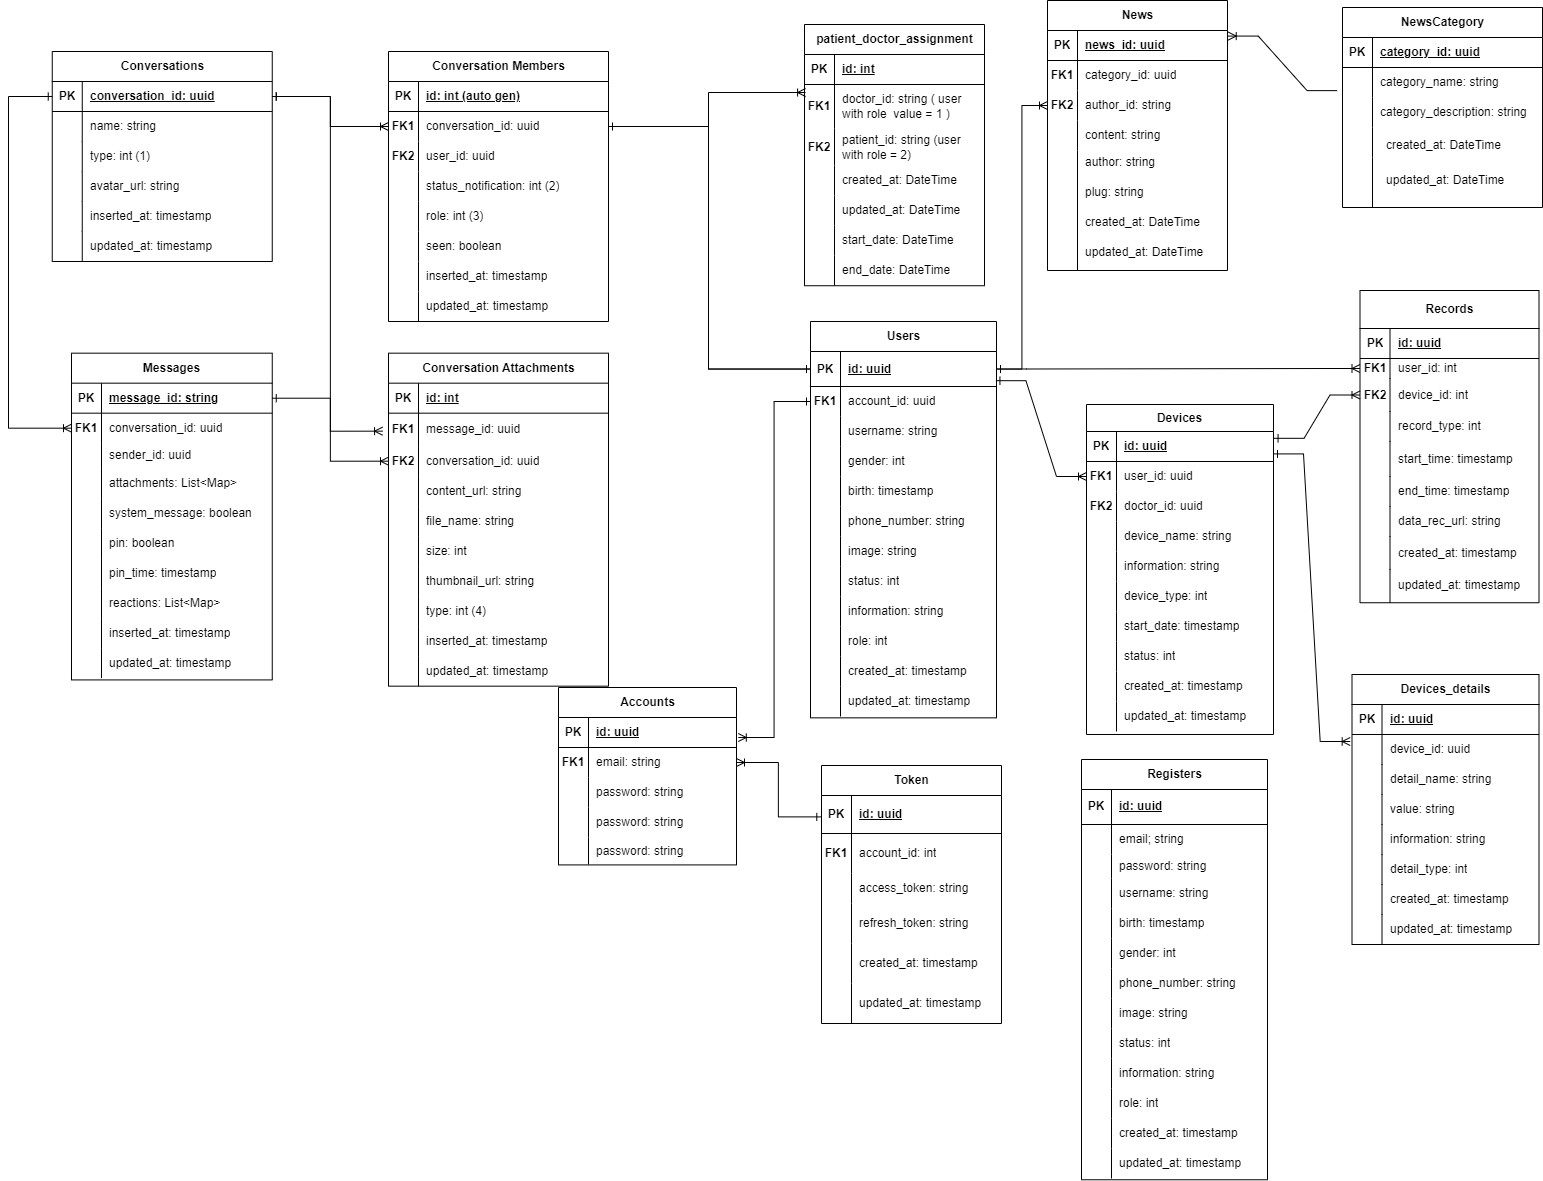
\includegraphics[width=15cm,height=15cm]{Images/system/fmECG_database.png}
%   \caption[Sơ đồ ERD]{\bfseries \fontsize{12pt}{0pt}\selectfont Sơ đồ ERD}
%   \label{fmECG_architecture-Database} %đặt tên cho ảnh
% \end{figure}

\subsection{Thiết kế giao diện}

\subsection{Thiết kế các chức năng cho website và server}

\subsubsection{Thiết kế API}


% \begin{enumerate}[a)]
%   \item API xác thực người dùng

%   \begin{xltabular}{\textwidth}{
%     | >{\raggedright\arraybackslash}p{4.5cm}
%     | >{\centering\arraybackslash}m{2.8cm}
%     | >{\raggedright\arraybackslash}X |
%     }
%     \caption{\bfseries \fontsize{12pt}{0pt}\selectfont Bảng API xác thực người dùng}
%     \label{table_api_auth}
%     \\
%     \hline
%     \bfseries Đường dẫn    &\bfseries Phương thức    &\bfseries Mô tả\\ \hline
%     api/auth/register   &   POST  & Đăng ký tài khoản \\ \hline
%   api/auth/login   &    POST    & Đăng nhập vào hệ thống \\ \hline
%   api/auth/logout   &    POST    & Đăng xuất khỏi hệ thống \\ \hline
%   api/auth/reset-password  &     POST   &  Gửi reset link kèm reset token đến email của người dùng để thay đổi mật khẩu \\  \hline
%   api/auth/reset-password/reset &   POST     &  Thay đổi lại mật khẩu với mã token được nhận  \\ \hline
%   \end{xltabular}

%   \item API xét duyệt đăng ký tài khoản

%   \begin{xltabular}{\textwidth}{
%     | >{\raggedright\arraybackslash}p{4cm}
%     | >{\centering\arraybackslash}m{2.8cm}
%     | >{\raggedright\arraybackslash}X |
%     }
%     \caption{\bfseries \fontsize{12pt}{0pt}\selectfont Bảng API xét duyệt đăng ký tài khoản}
%     \label{table_api_register}
%     \\
%     \hline
%     \bfseries Đường dẫn    &\bfseries Phương thức    &\bfseries Mô tả\\ \hline
%     api/register/list   &   GET  & Lấy danh sách các tài khoản đang chờ phê duyệt \\ \hline
%     api/register/accepted   &    POST    & Phê duyệt tài khoản đăng ký \\ \hline
%     api/register/rejected  &     POST   &  Từ chối phê duyệt tài khoản đăng ký \\  \hline  
%   \end{xltabular}

%   \item API quản lý thông tin người dùng
  
%   \begin{xltabular}{\textwidth}{
%     | >{\raggedright\arraybackslash}p{4cm}
%     | >{\centering\arraybackslash}m{2.8cm}
%     | >{\raggedright\arraybackslash}X |
%     }
%     \caption{\bfseries \fontsize{12pt}{0pt}\selectfont Bảng API quản lý thông tin người dùng}
%     \label{table_api_user}
%     \\
%     \hline
%     \bfseries Đường dẫn    &\bfseries Phương thức    &\bfseries Mô tả\\ \hline
%     api/user   &   GET  &  Lấy danh sách thông tin của tất cả người dùng \\  \hline
%    api/user/id/:userId  &   GET     & Lấy thông tin cụ thể của người dùng theo Id \\ \hline
%    api/user/role/:role  &   GET     & Lấy danh sách người dùng theo chức vụ \\ \hline
%    api/user/update   &    POST    &  Cập nhật thông tin người dùng \\  \hline
%    api/user/delete/:userId  &   DELETE     & Xóa thông tin người dùng theo Id \\ \hline
%   \end{xltabular}

% \item API quản lý thiết bị
% \begin{xltabular}{\textwidth}{
%   | >{\raggedright\arraybackslash}p{4.8cm}
%   | >{\centering\arraybackslash}m{2.8cm}
%   | >{\raggedright\arraybackslash}X |
%   }
%   \caption{\bfseries \fontsize{12pt}{0pt}\selectfont Bảng API quản lý thiết bị}
%   \label{table_api_device}
%   \\
%   \hline
%   \bfseries Đường dẫn    &\bfseries Phương thức    &\bfseries Mô tả\\ \hline
%   api/device   &   GET  & Lấy danh sách thông tin tất cả thiết bị \\ \hline
%   api/devide/:deviceId   &    GET    & Lấy thông tin của một thiết bị \\ \hline
%   api/device/add &   POST     & Thêm thông tin thiết bị mới \\ \hline
%   api/device/update  &     POST   & Cập nhật thông tin một thiết bị \\ \hline
%   api/device/delete/:deviceId  &     DELETE   & Xóa thông tin một thiết bị theo Id \\ \hline
% \end{xltabular}

% \item API quản lý bản ghi ECG
% \begin{xltabular}{\textwidth}{
%   | >{\raggedright\arraybackslash}p{5cm}
%   | >{\centering\arraybackslash}m{2.8cm}
%   | >{\raggedright\arraybackslash}X |
%   }
%   \caption{\bfseries \fontsize{12pt}{0pt}\selectfont Bảng API quản lý bản ghi ECG}
%   \label{table_api_ecg}
%   \\
%   \hline
%   \bfseries Đường dẫn    &\bfseries Phương thức    &\bfseries Mô tả\\ \hline
%  api/record   &   GET  & Lấy danh sách thông tin các phiên đo ECG \\ \hline
%  api/record/user/:userId   &    GET    & Lấy danh sách thông tin các phiên đo ECG của bệnh nhân \\ \hline
%  api/record/doctor/:doctorId &   GET     & Lấy danh sách thông tin các phiên đo ECG của các bệnh nhân được quản lý bởi bác sĩ \\ \hline
%  api/record/id/:recordId  &     GET   & Lấy thông tin một phiên đo của bệnh nhân \\ \hline
%  api/record/getData/:recordId  &     GET   & Lấy dữ liệu một phiên đo của bệnh nhân \\ \hline
%  api/ record/download/:recordId  &     GET   & Tải dữ liệu một phiên đo của bệnh nhân \\ \hline
%  api/record/update  &     POST   & Cập nhật thông tin một phiên đo của bệnh nhân \\ \hline
%  api/record/delete/:recordId  &     DELETE   & Xóa thông tin một phiên đo của bệnh nhân \\ \hline
%   \end{xltabular}


% \item API quản lý phân công bệnh sĩ - bệnh nhân
% \begin{xltabular}{\textwidth}{
%   | >{\raggedright\arraybackslash}p{4.5cm}
%   | >{\centering\arraybackslash}m{2.8cm}
%   | >{\raggedright\arraybackslash}X |
%   }
%   \caption{\bfseries \fontsize{12pt}{0pt}\selectfont Bảng API quản lý phân công bác sĩ - bệnh nhân}
%   \label{table_api_pda}
%   \\
%   \hline
%   \bfseries Đường dẫn    &\bfseries Phương thức    &\bfseries Mô tả\\ \hline
%   api/pda   &   GET  & Lấy danh sách tất cả thông tin phân công bác sĩ - bệnh nhân \\ \hline
%   api/pda/create  &    POST    & Tạo một phân công bác sĩ - bệnh nhân mới \\ \hline
%   api/pda/update  &    POST    & Cập nhật thông tin một phân công bác sĩ - bệnh nhân mới \\ \hline
%   api/pda/delete/:pdaId  &    DELETE    & Xóa một phân công bác sĩ - bệnh nhân mới \\ \hline
%   api/pda/patient/:doctorId &  GET  & Lấy danh sách tất cả bệnh nhân theo ID bác sĩ \\ \hline
%   api/pda/doctor/:patientId &  GET  & Lấy danh sách tất cả bác sĩ theo ID bệnh nhân \\ \hline
%   \end{xltabular}

% \end{enumerate}




\subsubsection{Sơ đồ tuần tự API}

% ------------------------Auth----------------------



\subsection{Kết luận chương}

Chương 3 trình bày chi tiết về quá trình thiết kế hệ thống, bao gồm kiến trúc tổng thể và các thành phần cụ thể. 
Thiết kế hệ thống tập trung vào việc xây dựng kiến trúc vận hành hiệu quả và mượt mà, chú trọng vào tính bảo mật, hiệu suất và khả năng mở rộng tối ưu.
\newpage